\documentclass{article}
\usepackage{amsmath}
\usepackage{amssymb}
\usepackage[pdftex]{graphicx}
\usepackage[framed,numbered,autolinebreaks,useliterate]{mcode}
\lstset{breakatwhitespace=false}
\usepackage{pgfplots}

\pdfpagewidth 8.5in
\pdfpageheight 11in
\topmargin -1in
\headheight 0in
\headsep 0in
\textheight 8.5in
\textwidth 6.5in
\oddsidemargin 0in
\evensidemargin 0in 
\headheight 50pt
\headsep 0in
\footskip .75in

\title{STA 601 - Lab 8}
\author{Kedar Prabhudesai}
\date{November 8, 2013}

\begin{document}
\maketitle

\noindent {\underline{\textbf{Data Likelihood:}}}\\
\begin{eqnarray*}
L(x;\mu,\sigma) = \prod_{i=1}^{n}{\frac{1}{x_i\sigma \sqrt{2\pi}}exp\left[\frac{-(ln x_i-\mu)^2}{2\sigma^2}\right]}
\end{eqnarray*}
\begin{center}
Let $\tau = 1/\sigma^2$\\
\end{center}
\begin{eqnarray*}
L(x;\mu,\tau) &=& \prod_{i=1}^{n}{\frac{\sqrt{\tau}}{x_i\sqrt{2\pi}}exp\left[\frac{-\tau(ln x_i-\mu)^2}{2}\right]}\\
\therefore L(x;\mu,\tau) &=& \frac{\tau^{n/2}}{x_i^n2\pi^{n/2}}exp\left[-\frac{\tau}{2}\sum_{i=1}^{n}{(ln x_i-\mu)^2}\right]\\
\end{eqnarray*}

\noindent {\underline{\textbf{Priors:}}}\\
\begin{eqnarray*}
\mu &\sim& \mathcal{N}(\mu_0,\tau_0)
\therefore p(\mu) = \frac{\sqrt{\tau_0}}{\sqrt{2\pi}}exp\left[\frac{-\tau_0(\mu-\mu_0)^2}{2}\right]\\
\tau &\sim& Gamma(\alpha,\beta)
\therefore p(\tau) = \frac{\beta^\alpha}{\Gamma(\alpha)}\tau^{\alpha-1}exp(-\beta\tau)
\end{eqnarray*}

\noindent {\underline{\textbf{Posterior:}}}\\
\begin{eqnarray*}
p(\mu,\tau \mid x) &\propto& L(x;\mu,\tau) \times p(\mu) \times p(\tau)\\
\therefore p(\mu,\tau \mid x) &\propto& \frac{\tau^{n/2}}{x_i^n}exp\left[-\frac{\tau}{2}\sum_{i=1}^{n}{(ln x_i-\mu)^2}\right] \times \sqrt{\tau_0}exp\left[\frac{-\tau_0(\mu-\mu_0)^2}{2}\right] \times \tau^{\alpha-1}exp(-\beta\tau)
\end{eqnarray*}

\pagebreak

\noindent {\underline{\textbf{Full Conditionals:}}}\\
\begin{eqnarray*}
p(\mu \mid \tau,x) &\propto& exp\left[-\frac{\tau}{2}\sum_{i=1}^{n}{(ln x_i-\mu)^2} - \frac{\tau_0}{2}(\mu-\mu_0)^2\right]\\
p(\tau \mid \mu,x) &\sim& Gamma\left(\alpha + \frac{n}{2},\frac{\sum_{i=1}^{n}{(ln x_i-\mu)^2}}{2}+\beta\right)
\end{eqnarray*}

In our Gibbs Sampler, we update $\mu$ using Metropolis-Hastings and $\tau$ using the Gamma Distribution.\\

\noindent {\underline{\textbf{Gibbs Sampler:}}}\\

Start with \{\mu^{(0)}\}

\begin{itemize}
\item Sample, $\mu' \sim \mathcal{N}(\mu^{(s)},\sigma_{cand})$
\item Compute acceptance ratio, $r = p(\mu' \mid \tau^{(s)},x)/p(\mu \mid \tau^{(s)},x)$
\item Draw, $u \sim$ Uniform[$0,1$]. If $u < r,$ $\mu^{(s+1)} = \mu'$, else $\mu^{(s+1)} = \mu^{(s)}$.
\item Sample, $\tau^{(s+1)} \sim p(\tau \mid \mu^{(s+1)},x)$
\end{itemize}

\noindent {\underline{\textbf{Posterior Predictive:}}}
\begin{eqnarray*}
p(x_{n+1} \mid x_1,x_2,\ldots,x_n) &=& \int{\int{p(x_{n+1} \mid \mu,\tau)p(\mu,\tau \mid x_1,x_2,\ldots,x_n)d\mu}d\tau}
\end{eqnarray*}
We can sample from the posterior predictive using Monte-Carlo procedure. Use $\{\mu^{(s)},\tau^{(s)}\}$ samples from the Gibbs Sampler and sample from $x^{(s)} \sim p(x \mid \mu^{(s)},\tau^{(s)})$. Then posterior predictive can be approximated as, $p(x_{n+1} \mid x_1,x_2,\ldots,x_n) = \frac{\sum_{s=1}^{S}{x^{(s)}}}{S}.$

\pagebreak
\noindent {\underline{\textbf{Weekday Prior Values:}}}\\
Prior parameters for $\mu_1$: $\mu_0 = 0.6, \tau_0 = 400.$\\
Prior parameters for $\tau_1$: $\alpha = 1, \beta = 20.$\\

\noindent {\underline{\textbf{Weekend Prior Values:}}}\\
Prior parameters for $\mu_2$: $\mu_0 = 0.2, \tau_0 = 400.$\\
Prior parameters for $\tau_2$: $\alpha = 1, \beta = 20.$\\

We verify that, $P(\mu_1 > \mu_2) = 1.$ This is comparison of the two priors.
\begin{center}
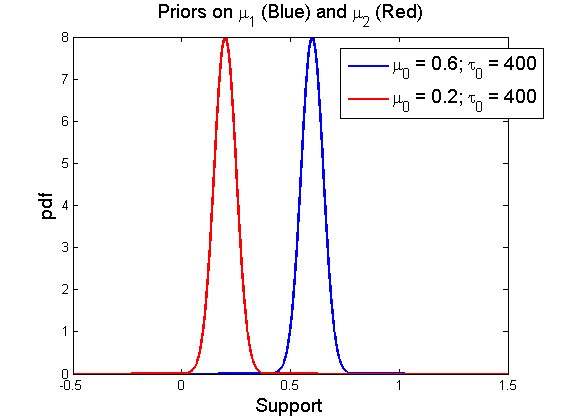
\includegraphics[scale=0.75]{mu1mu2Priors.png}\\
\end{center}

\pagebreak
\noindent {\underline{\textbf{Sampling Results:}}}\\

Following are trace plots for $\mu_1$ and $\sigma_1^2.$\\

\begin{center}
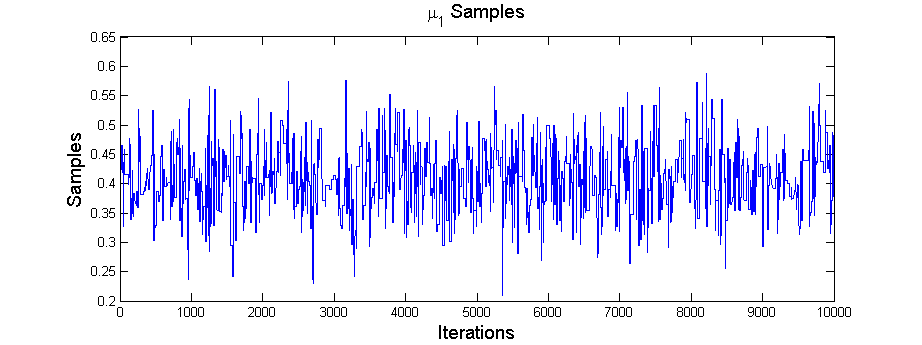
\includegraphics[scale=0.75]{mu1Samples.png}\\
\end{center}

\begin{center}
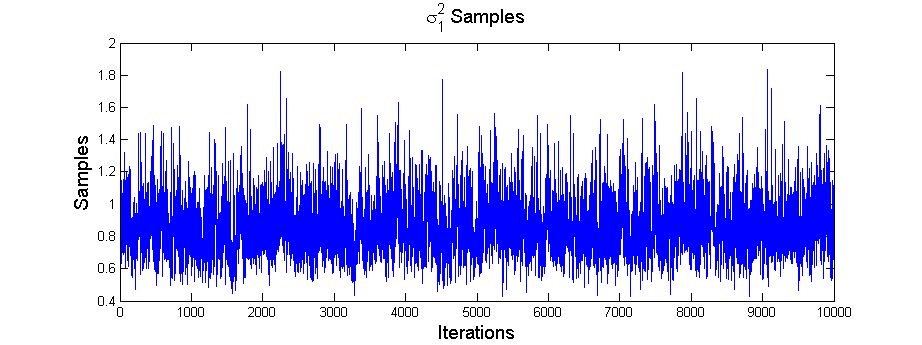
\includegraphics[scale=0.75]{S12Samples.png}\\
\end{center}

\noindent {\underline{\textbf{Estimates and 95\% Credible Intervals:}}}\\
$\mu_1 \rightarrow 0.4102$ [$0.3037,0.5219$].\\
$\sigma_1^2 \rightarrow  0.8585$ [$0.5750,1.2491$].\\
$\mu_2 \rightarrow  0.1533$ [$0.0462,0.2561$].\\
$\sigma_2^2 \rightarrow 2.4503$ [$1.4273,4.1320$].\\

\noindent {\underline{\textbf{Probabilities of Interest:}}}\\
Posterior $P(\mu_1 > \mu_2) = 0.9998.$ Posterior $P(\sigma_1 > \sigma_2) =  0.0012.$\\
Posterior Predictive, $P(x_{n+1}^{Weekday} > x_{n+1}^{Weekend} \mid x_1,x_2,\ldots,x_n) =  0.5470.$\\

\pagebreak
\noindent {\Large\underline{\textbf{Appendix:}}}\\
\lstinputlisting{C:/Users/ksp6/Documents/Classes/2013-Fall/STA601-BayesAndModStats/labs/lab8/sta601_ksp6_Lab8.m}

\end{document}